\pentry{\textbf{预备知识\ }矩阵\upref{Mat},绕轴旋转的线速度 %未完成:引用
}
\subsection{结论}
直角坐标系中,某点 $\vec r=(x,y,z)\Tr$ 以单位矢量 $\uvec A=({A_x},{A_y},{A_z})\Tr$ 为轴按右手定则%未完成 链接
转动 $\theta$ 角的得到的点 $\vec r'=(x',y',z')\Tr$ 可用矩阵乘法计算
\begin{equation}
\vec r' = {\mat R_\theta }\vec r
\end{equation}
其中 $\mat R_\theta$ 为\textbf{绕轴旋转矩阵}
\begin{equation}
\mat R_\theta =
\begin{pmatrix}
\eta A_x^2 + \cos\theta & \eta A_x A_y - A_z\sin\theta & \eta A_x A_z + A_y\sin\theta\\
\eta A_y A_x + A_z\sin\theta & \eta A_y^2 + \cos\theta & \eta A_y A_z - A_x\sin\theta\\
\eta A_z A_x - A_y \sin\theta & \eta A_z A_y + A_x\sin\theta & \eta A_z^2 + \cos\theta
\end{pmatrix}\end{equation}

\subsection{推导}
推导的思路是用 $\uvec A$ , $\vec r$ 和 $\theta $ 三个以质量经过数乘,点乘\upref{Dot}和叉乘\upref{Cross}三种运算,表示出旋转后的矢量 $\vec r'$,再拆成三个分量,即可得到线性变换,进而写出矩阵. 注意该思路与推导平面旋转矩阵\upref{Rot2D} 的思路不一样.
\begin{figure}[h]
\centering
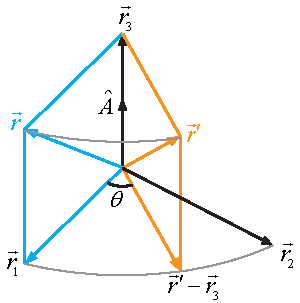
\includegraphics[width=5cm]{./figures/RotA.pdf}
\caption{图 1}
\end{figure} 

如图, $\vec r$ 绕单位矢量 $\uvec A$ 旋转后得到 $\vec r'$ .  $\vec r$ 在 $\uvec A$ 方向的分量为   
\begin{equation}\label{RotA_eq1}
{\vec r_3} = (\uvec A \vdot \vec r)\uvec A
\end{equation}
 在与 $\uvec A$ 垂直方向的分量为
\begin{equation}\label{RotA_eq2}
{\vec r_1} = \vec r - {\vec r_3}
\end{equation}
 为了构成一组正交基底,令
 \begin{equation}\label{RotA_eq3}
{\vec r_2} = \uvec A \cross {\vec r_1}
\end{equation}
则 ${\vec r_2}$ 相当于 ${\vec r_1}$ 绕 $\uvec A$ 旋转 90°. 现在有了正交的 ${\vec r_1}$ , ${\vec r_2}$  就可以表示出 ${\vec r_1}$ 绕 旋转 $\theta $ 角后的结果
\begin{equation}
\vec r' - {\vec r_3} = {\vec r_1}\cos \theta  + {\vec r_2}\sin \theta
\end{equation}
即
\begin{equation}\label{RotA_eq4}
\vec r' = {\vec r_1}\cos \theta  + {\vec r_2}\sin \theta  + {\vec r_3}
\end{equation} 
将式\eqref{RotA_eq1}\eqref{RotA_eq2}\eqref{RotA_eq3}代入\eqref{RotA_eq4},即可求出 $\vec r'$ 关于 $\uvec A$ , $\vec r$ 和 $\theta $ 的矢量表达式. 把结果写成分量的形式,化简可得到 $x',y',z'$ 关于 $x,y,z$ 的线性变换与系数矩阵\upref{Mat}.

\subsection{由旋转矩阵推导出匀速圆周运动的线速度} 

虽然这个公式有更简单的几何方法(见绕轴旋转的线速度%未完成:词条 引用
),但是这种方法更偏数学一些,也验证了旋转矩阵的正确性.

在无穷小的时间 $t$ 内,点 $P$ 绕轴转过 $\theta $ 角,则 $\theta  = \omega t \to 0$, 此时有 $\sin\theta  \to \theta $ 和 $\cos \theta  \to 1$ . 旋转矩阵变为
\begin{equation}
\mat R_\theta =
\begin{pmatrix}
{1}&{ - {A_z}\theta }&{{A_y}\theta }\\
{{A_z}\theta }&1&{ - {A_x}\theta }\\
{ - {A_y}\theta }&{{A_x}\theta }&1
\end{pmatrix}
\end{equation}
下面 $\mat R_\theta$ 乘以某点的列矢量,得到变换后的坐标,再减掉变换前的坐标,得位移矢量 $\vec s$
\begin{equation}\begin{split}
\vec s &= \vec v t\\
&= \pmat{1 & -A_z\theta & A_y\theta\\A_z\theta & 1 & -A_x\theta\\-A_y\theta & A_x\theta & 1} \pmat{x\\y\\z}
-\pmat{1&&\\&1&\\&&1} \pmat{x\\y\\z}\\
&= \theta \pmat{0 & -A_z & A_y\\A_z & 0 & -A_x\\-A_y & A_x & 0}\pmat{x\\y\\z}\\
&= \theta\uvec A\cross\vec r\\
&= \left(\vec \omega t\right) \cross \vec r
\end{split}\end{equation} 
两边除以 $t$,得 $\vec v = \vec \omega  \cross \vec r$ 这与绕轴转动的线速度% 未完成
中得出的结论一致.